%%%%%%%%%%%%%%%%%%%%%%%%%%%%%%%%%%%%%%%%%
% Template
% LaTeX Template
% Version 1.0 (December 8 2014)
%
% This template has been downloaded from:
% http://www.LaTeXTemplates.com
%
% Original author:
% Brandon Fryslie
% With extensive modifications by:
% Vel (vel@latextemplates.com)
%
% License:
% CC BY-NC-SA 3.0 (http://creativecommons.org/licenses/by-nc-sa/3.0/)
%
% Authors:
% Sabbir Ahmed
% 
%%%%%%%%%%%%%%%%%%%%%%%%%%%%%%%%%%%%%%%%%

\documentclass[paper=usletter, fontsize=12pt]{article}
%%%%%%%%%%%%%%%%%%%%%%%%%%%%%%%%%%%%%%%%%
% Contract Structural Definitions File Version 1.0 (December 8 2014)
%
% Created by: Vel (vel@latextemplates.com)
% 
% This file has been downloaded from: http://www.LaTeXTemplates.com
%
% License: CC BY-NC-SA 3.0 (http://creativecommons.org/licenses/by-nc-sa/3.0/)
%
%%%%%%%%%%%%%%%%%%%%%%%%%%%%%%%%%%%%%%%%%

\usepackage{geometry} % Required to modify the page layout
\usepackage{multicol}
\usepackage{amsmath}
\usepackage{amssymb}

\usepackage[pdftex]{graphicx}
\usepackage{wrapfig}
\usepackage[font=scriptsize, labelfont=bf]{caption}
\usepackage[utf8]{inputenc} % Required for including letters with accents
\usepackage[T1]{fontenc} % Use 8-bit encoding that has 256 glyphs

\usepackage{avant} % Use the Avantgarde font for headings
\usepackage{courier}
\usepackage{xparse}
\usepackage{xcolor}
\usepackage{listings}  % for code verbatim and console outputs

\setlength{\textwidth}{16cm} % Width of the text on the page
\setlength{\textheight}{23cm} % Height of the text on the page
\setlength{\oddsidemargin}{0cm} % Width of the margin - negative to move text left, positive to move it right
\setlength{\topmargin}{-1.25cm} % Reduce the top margin

\setlength{\parindent}{0mm} % Don't indent paragraphs
\setlength{\parskip}{2.5mm} % Whitespace between paragraphs
\renewcommand{\baselinestretch}{1.5}

\definecolor{green}{rgb}{0.18, 0.55, 0.34}

\graphicspath{ {figures/} }
\captionsetup[table]{skip=10pt}

\lstset{language=C, keywordstyle={\bfseries \color{black}}}

% defines algorithm counter for chapter-level
\newcounter{nalg}[section]

%defines appearance of the algorithm counter
\renewcommand{\thenalg}{\thesection .\arabic{nalg}}

% defines a new caption label as Algorithm x.y
\DeclareCaptionLabelFormat{algocaption}{Algorithm \thenalg}

% defines the algorithm listing environment
\lstnewenvironment{pseudocode}[1][] {
    \refstepcounter{nalg}  % increments algorithm number
    \captionsetup{font=normalsize, labelformat=algocaption, labelsep=colon}
    \lstset{
        breaklines=true,
        mathescape=true,
        numbers=left,
        numberstyle=\scriptsize,
        basicstyle=\footnotesize\ttfamily,
        keywordstyle=\color{black}\bfseries,
        keywords={input, output, return, parallel, function, for, to, in, if,
        else, foreach, while, and, or, new, print},
        xleftmargin=.04\textwidth,
        #1
    }
}{}

\renewcommand{\familydefault}{\sfdefault}  % default font for entire document
 % specifies the document layout and style

\begin{document}

    \documentinfo{\textbf{Homework 4: Snake Preliminary Design}}{\today}{Sabbir Ahmed}
    \vspace{-0.1in}

    \section{Background}
    For this assignment, a version of the classical snake game will be implemented.

    % The game was to conform to the following specifications:

    % \begin{itemize}

    %     \item The game play area is set up as a 26-by-38 grid surrounded by an electric fence (blue). The game display should occupy the majority of the screen.

    %     \item To start the game, press RESET/BTN\_SOUTH. Upon release, a single grid point represents a snake (green) and a single grid point represents food (red).

    %     \item The snake starts by moving to the right one grid point roughly every 1/8th of a second (125 ms update interval).

    %     \item A player may change the direction of the movement by 90 degree clockwise or counterclockwise by using the rotary switch on the FPGA board. Every position (notch) change of the rotary switch should correspond to a 90 degree angle change.

    %     \item If the snake goes onto the fence, the game should freeze.

    %     \item If the snake goes onto the food, the length of the snake should increase by one grid segment on the next movement with a trailing body, per the behavior of the game shown in the provided link. The moving head be green, and the grown body should be cyan (green+blue).

    %     \item Each time the snake reaches the food, another food should be positioned in a manor seemly random to the user.

    %     \item Each subsequent time the snake eats food, the segment length should grow by one, up to a length of 32 (including the head).

    %     \item If the head of the snake overlaps a body segment then the game should freeze.

    %     \item If the length of the snake reaches 32, the game should instead increase in speed by reducing the update interval by roughly 10 ms.

    % \end{itemize}

    \section{Design Approach}
    Several discrete modules will be used to implement the game: \inlsnip{rotary_oneshot}, \inlsnip{direction} \inlsnip{snake_pos}, \inlsnip{food_pos}, \inlsnip{collision}, \inlsnip{pacemaker} and \inlsnip{vga_layout}. These submodules will be connected using a top level module that may be visualized with the schematic diagram configured as a block diagram in Figure \ref{fig:schematic}. All the modules implicitly accept clock cycles as inputs.

    \begin{figure}[ht]
        \begin{center}
            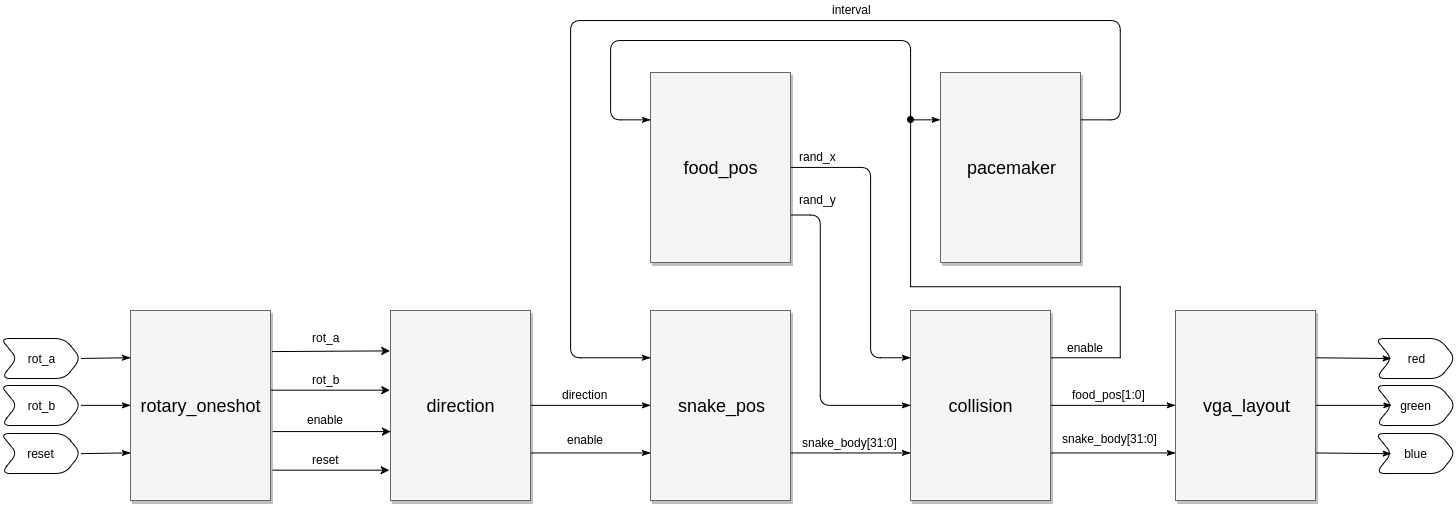
\includegraphics[width=1\textwidth]{top_level_design.png}
            \caption{Schematic of the Implementation of the Game} \label{fig:schematic}
        \end{center}
    \end{figure}
    \newpage

        \subsection{direction and rotary\_oneshot}
        The \inlsnip{rotary_oneshot} and \inlsnip{direction} modules will both be used as to control the user inputs.

        \inlsnip{rotary_oneshot} directly handles the user inputs, \texttt{rot\_a}, \texttt{rot\_b} and \texttt{reset}. The inputs are one-shotted and passed to \inlsnip{direction} to determine the direction the user intended. This module sets an enable to the \inlsnip{snake_pos} module to notify a change in direction.

        \subsection{snake\_pos}
        The \inlsnip{snake_pos} module generates the coordinates for the 32 segments of the snake body, including its head. The module takes in the 2 bit direction and 1 bit enable inputs from \inlsnip{direction}. It also accepts the \texttt{interval} input from \inlsnip{pacemaker} to determine the speed of the moving snake body.

        \subsection{food\_pos}
        This module generates the \texttt{rand\_x} and \texttt{rand\_y} coordinates of the food when enabled by the \inlsnip{collision} module.

        \subsection{collision and pacemaker}
        \inlsnip{collision} accepts the coordinates of the food and the snake segments and determines if a collision has been detected. If a collision has not been detected, it sends out an enable signal to the \inlsnip{snake_pos} module. If a collision with the snake body, specifically the snake head, with the food is detected, the module sends a signal to \inlsnip{pacemaker} to determine the interval at which the snake should move. This module has an internal counter that speeds up when the snake head had made 32 collisions with the food. If a collision between the snake head and the fence is detected, the game is frozen.

        \subsection{vga\_layout}
        This module draws the fence of the game, and the snake and the randomly placed food on the VGA display.

    \section{Test Plan and Methodology}
    Individual modules are being built sequentially. A testbench to accompany those modules are also being built concurrently. The sequence at which the modules are being tested and built can be outlined by the block diagram going from left to right. The leftmost modules are being built and tested before their proceeding modules, with the exception of \inlsnip{vga_layout} which required extensive testing to be able to withstand all its dependencies.
    %     The \inlsnip{igniter} submodule allowed the player to interface with the LEDs. It accepted the 4 switches as the input, representing them as the 4 bit \inlsnip{delta} of the current position of the user. The submodule also handled BTN\_NORTH, acting as the enable.

    %     A testbench has been included with the project to demonstrate usage of the submodule and its effects on the position of the player in \inlsnip{igniter_tb}. A sample waveform output has been provided:

    %     \begin{figure}[ht]
    %         \begin{center}
    %             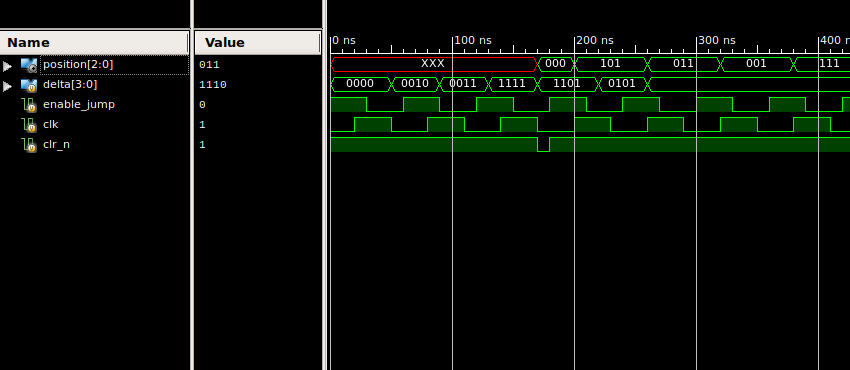
\includegraphics[width=1\textwidth]{igniter_wav.png}
    %             \caption{Waveform of the Testbench of igniter} \label{fig:igniter_wav}
    %         \end{center}
    %     \end{figure}
    %     \newpage

    %     \subsection{extinguisher}
    %     The \inlsnip{extinguisher} submodule turns the LEDs off using a pseudo-random index generator. It consists of an internal counter, running independently of the rest of the submodule on each clock cycle. The 4 bit counter iterates through all its 16 states, and outputs an active signal when the module is enabled. The active signal outputs high when the counter is less than 8 and assigns the value to the index of the LED to be turned off.

    %     The 50 MHz clock speed from the development board cycles through the counter very rapidly: 

    %      \[ 50 \ MHz=\frac{1}{50 \times 10^{6}} \ s=20 \ ns \times 16 \ states = \frac{1 \ counter \ loop}{320 \ ns} \]

    %     This speed allows the player to perceive the outputs of the submodule to be random.

    %     A testbench has been included with the project to demonstrate usage of the submodule and its effects on the position of the player in \inlsnip{extinguisher_tb}. A sample waveform output has been provided:

    %     \begin{figure}[ht]
    %         \begin{center}
    %             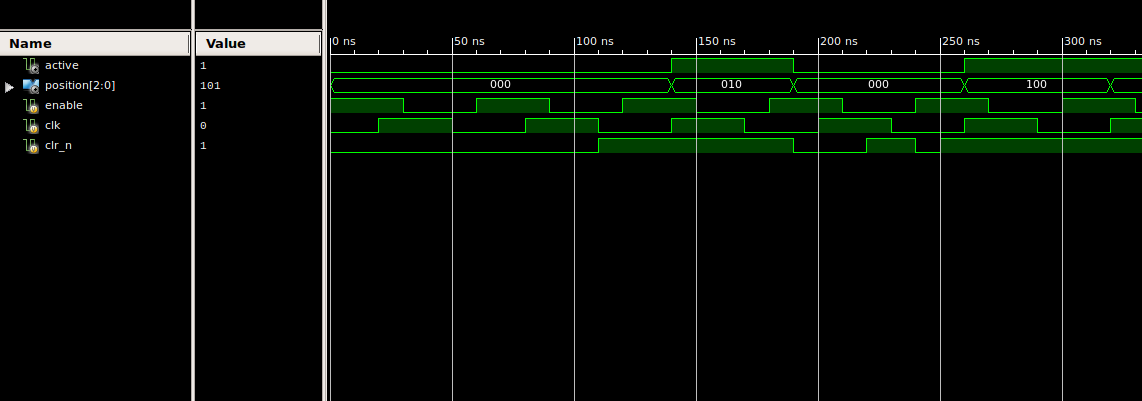
\includegraphics[width=1\textwidth]{extinguisher_wav.png}
    %             \caption{Waveform of the Testbench of extinguisher} \label{fig:extinguisher_wav}
    %         \end{center}
    %     \end{figure}
    %     \newpage

    %     \subsection{candle\_controller}

    %     The \inlsnip{candle_controller} submodule directly handles the states of the LED outputs. It utilizes the outputs from the other two submodules to determine the states of the individual LEDs.

    %     A testbench has been included with the project to demonstrate usage of the submodule and its effects on the position of the player in \inlsnip{candle_controller_tb}. A sample waveform output has been provided:

    %     \begin{figure}[ht]
    %         \begin{center}
    %             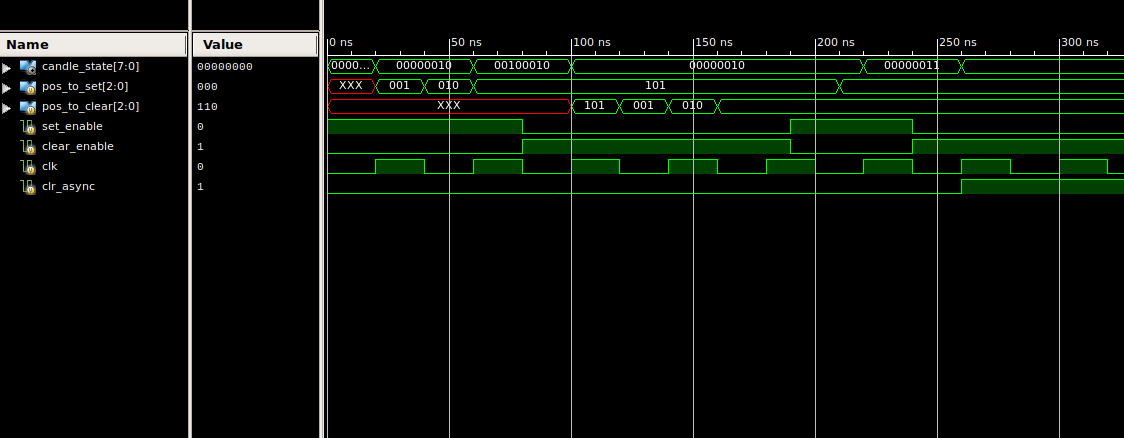
\includegraphics[width=1\textwidth]{candle_controller_wav.png}
    %             \caption{Waveform of the Testbench of candle\_controller} \label{fig:candle_controller_wav}
    %         \end{center}
    %     \end{figure}
    %     \newpage

    %     \subsection{Top Level Module}
    %     The top level module, \inlsnip{top.v}, connects all the submodules with wires. A testbench has also been included with the project to demonstrate the implementation of the game in \inlsnip{top_tb}. A sample waveform output has been provided:

    %     \begin{figure}[ht]
    %         \begin{center}
    %             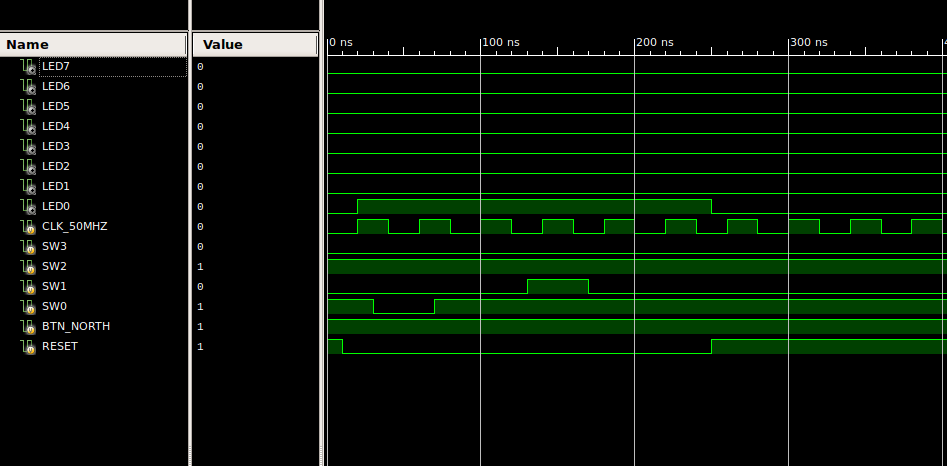
\includegraphics[width=1\textwidth]{top_wav.png}
    %             \caption{Waveform of the Testbench of top} \label{fig:top_wav}
    %         \end{center}
    %     \end{figure}

    % \section{Troubleshooting}
    % Several software and hardware issues were emphasized during the timeline of this assignment. Software glitches include the Xilinx ISE not being able to interface the development board at random times after successful synthesis. Hardware issues included the board not being able to properly process the switches as inputs in the initial stages of the assignment timeline.

    % \section{Results}
    % All the testbenches generated the expected outputs, and the project was successfully synthesized. The game was implemented on the board to an extent. The LEDs appear to be frozen in state when the BTN\_NORTH enable was pushed. The RESET button appear to work, but the inputs of the switches could not be validated because of the LEDs resisting to change their states.

\end{document}
